\documentclass{beamer}
\usepackage[utf8]{inputenc}
\usepackage[T1]{fontenc}
\usepackage{lmodern}
\usepackage[portuguese]{babel}
\usetheme{Berlin}
\definecolor{RoxoBeamer}{RGB}{81, 40, 136} 
\usecolortheme[named=RoxoBeamer]{structure}
\usepackage{amsmath}
\usepackage{amsfonts}
\usepackage{amssymb}
\usepackage{graphicx}
\usepackage{tikz}
\usepackage{siunitx}
\usepackage[style=abnt,backend=biber]{biblatex}                                                                                                  
\addbibresource{Congresso.bib}      

\title{A Escolha do Modelo como Decisão Axiomática: Misspecification e Fuzzy Time Series}
\author{Gabriel Gomes}
\institute{FATEC-RL}
\date{}

\begin{document}
	
	\maketitle
	
	\begin{frame}
		\begin{center}
			\Large \textit{``All models are wrong, but some are useful.''} \newline
			\normalsize	-George E. P. Box
		\end{center}
	\end{frame}
	
	\begin{frame}{O Caso-Problema: \textcite{santos2023porto}}
		
		\textcite{santos2023porto} analisam a movimentação de carga do Porto de Santos
		(2005--2022) e propõem um modelo de previsão para 2023--2026 baseado em
		\textbf{regressão linear simples}.
		
	\begin{figure}
		\centering
		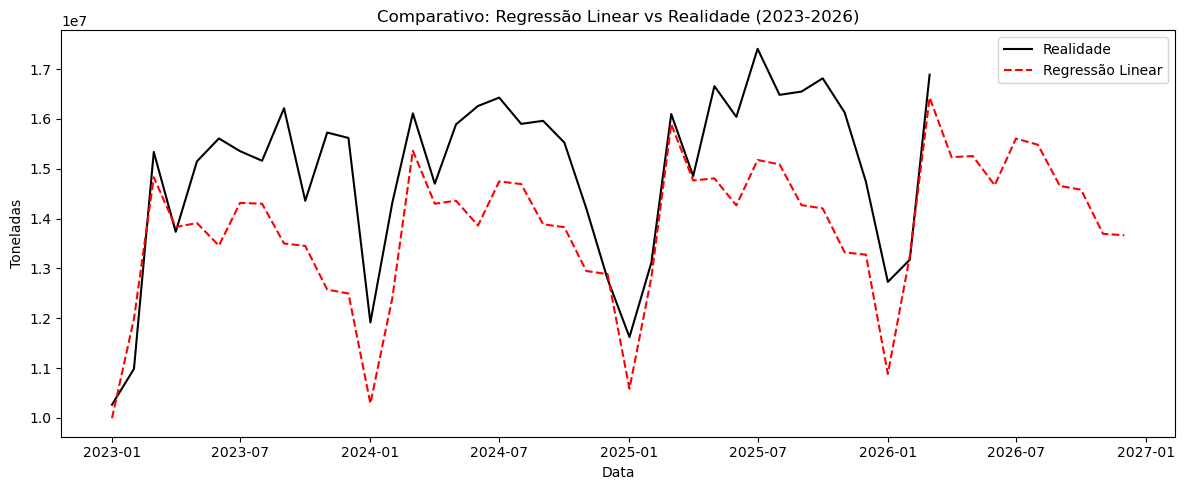
\includegraphics[width=1\linewidth]{Images/real_rl.png}
	\end{figure}
		
	\end{frame}
	
	\begin{frame}{A Simplicidade do Modelo como Motivação}
		
		Os autores justificam a escolha afirmando que, embora existam modelos
		mais adequados para séries temporais com sazonalidade (e.g., SARIMA),
		a regressão linear oferece:
		
		\vspace{5mm}
		
		\begin{quote}
			\textit{``[...] um modelo simples como a regressão linear em uma
				predição e realizando-o com um custo computacional muito menor.''}
			\hfill \parencite{santos2023porto}
		\end{quote}
		
		\vspace{5mm}
		
		Mas apelar à simplicidade sem especificar
		\textit{o que se perde} com a simplificação
		é uma justificativa \textbf{metodologicamente vazia}:
		ela não gera nenhum conteúdo testável independentemente
		\parencite{lakatos1970falsification}.
		
	\end{frame}
	
	\begin{frame}{A Estratégia dos 12 Modelos Mensais}
		
		Para contornar a sazonalidade, os autores treinaram
		\textbf{12 regressões lineares independentes} — uma para cada mês:
		
		\begin{figure}
			\centering
			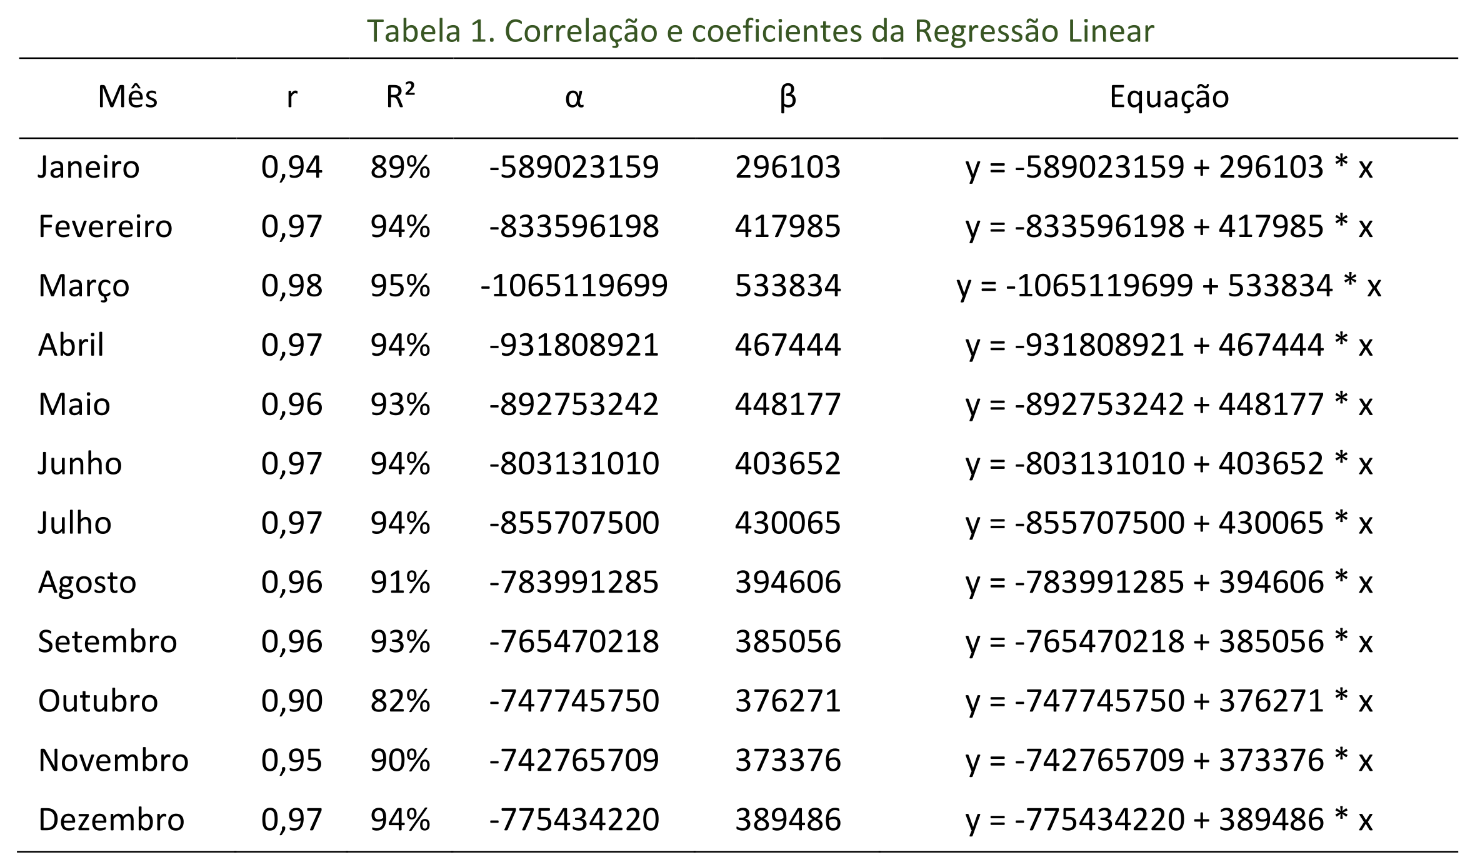
\includegraphics[width=0.9\linewidth]{Images/tabela.png}
		\end{figure}
		
	\end{frame}
	
		\begin{frame}{}
		
		\begin{quote}
			\textit{"Diante das correlações encontradas para cada uma das curvas individualizadas dos meses serem aceitáveis, bem como os coeficientes de determinação ($R^{2} \ge 80\%$), seguiu-se com a determinação da reta média da regressão linear."}
			\hfill \parencite{santos2023porto}
		\end{quote}
		
		\vspace{5mm}
		
		Os altos $R^2$ são apresentados como evidência de ``sucesso''
		do modelo — mas será isso suficiente?
		
	\end{frame}
	
	\begin{frame}{Regressão Espúria e Ajuste de Curva}                                                                                                                 
		\textcite{granger1974spurious} demonstram justamente esse padrão onde            nos modelos de Regressão Linear você podem ter coeficientes $R^{2}$ altos e ao mesmo tempo não passam no teste Durbin-Watson para autocorrelação, sendo esses modelos classificados como \textbf{Regressões Espúrias}.                                                               
		
		\vspace{1em}                                                                                                                                 
		Na concepção de \textcite{spanos2007curve}, o caso \textcite{santos2023porto} representa exatamente um problema de \textit{"Curve Fitting"} (Ajuste de Curva). Ao tratarem a solução através da métrica do coeficiente $R^{2}$, a avaliação de sucesso do modelo foi definida como \textit{“goodness-of-fit”} (Qualidade do Ajuste), em uma aplicação de 12 modelos com $R^{2}$ acima de $80\%$.
		
	\end{frame}
	
	
	\begin{frame}{Deborah Mayo e o Teste Severo}
		\begin{columns}[T,onlytextwidth]
			\begin{column}{0.35\textwidth}
				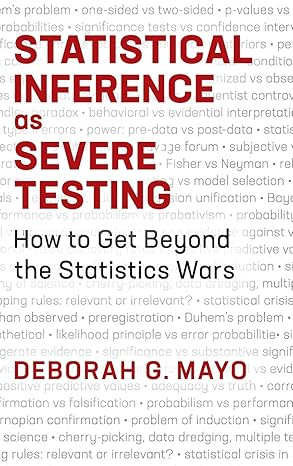
\includegraphics[width=\linewidth]{Images/Severe.jpg}
			\end{column}
			\begin{column}{0.60\textwidth}
				\begin{quote}
					\footnotesize\textit{``The growing availability of
						computer power and statistical software has greatly
						increased the ease with which practitioners apply
						statistical methods, but this has not been accompanied
						by attention to checking the assumptions on which these
						methods are based.[...]''}
					\hfill \parencite{mayo2004methodology}
				\end{quote}
				\vspace{0.3em}
				Este é o padrão que motiva o \textbf{teste severo}:
				Mayo \parencite{mayo2018statistical} propõe que uma inferência é
				bem sustentada apenas se o procedimento que a gerou
				provavelmente teria detectado $H$, caso $H$ fosse falsa.
			\end{column}
		\end{columns}
	\end{frame}
	
	\begin{frame}{{\small Mayo e as Duas Classes de Perguntas para Aplicação de um Modelo}}
		conteúdo...
	\end{frame}

	\begin{frame}{M-S Teste em \textcite{santos2023porto}}		
		\begin{figure}
			\centering
			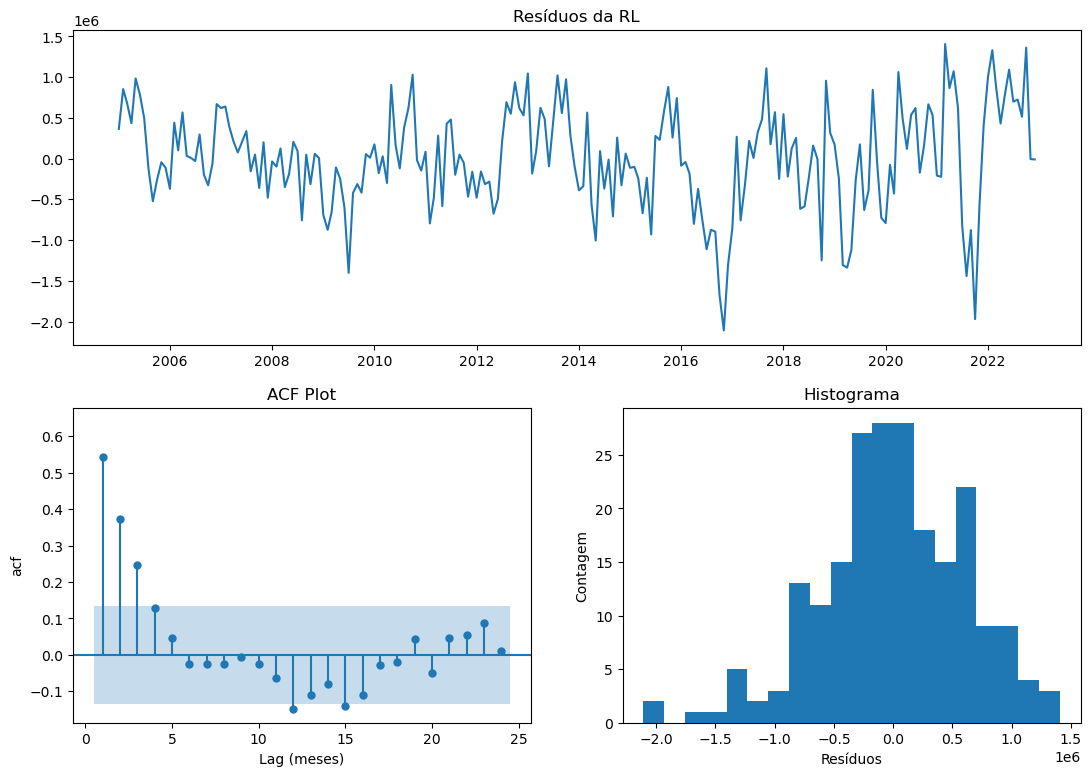
\includegraphics[width=0.9\linewidth]{Images/diag_rl.png}
		\end{figure}
		
	\end{frame}
	
	\begin{frame}
		A regressão linear pressupõe resíduos \textbf{independentes e
		identicamente distribuídos} ($\varepsilon_i \overset{\text{iid}}{\sim}
		\mathcal{N}(0, \sigma^2)$).
		
		\vspace{0.5em}
		
		O teste de Ljung-Box aplicado aos resíduos agregados
		($n = 216$, lags $= 12$) revela:
		
		\begin{block}{Resultado}
			$\text{LB}_{12} = 119{,}27, \quad p = 8{,}6 \times 10^{-20}$
		\end{block}
		\begin{figure}
			\centering
			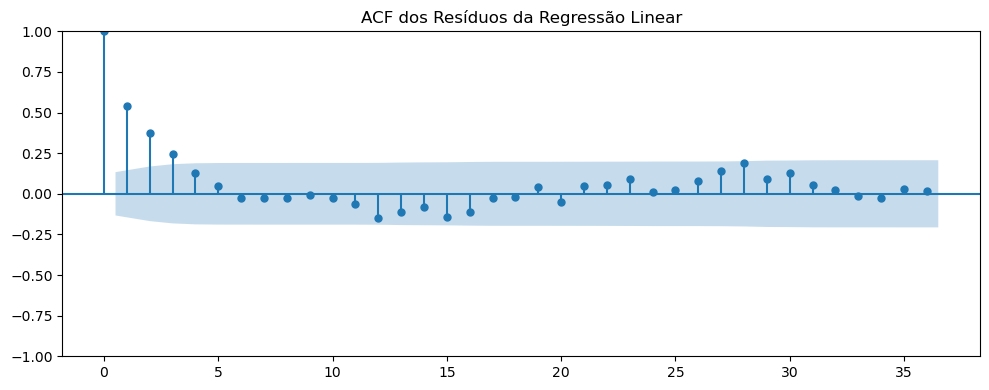
\includegraphics[width=0.9\linewidth]{Images/resid_rl.png}
		\end{figure}
		
	\end{frame}
	
	\begin{frame}{A Representação de um Fenômeno Maior}
		\begin{columns}[T]
			\begin{column}{0.35\textwidth}
				\centering
				\resizebox{\linewidth}{!}{\textit{6.1 - Why Not Use a Linear Regression?}}
				
				\vspace{0.2cm}
				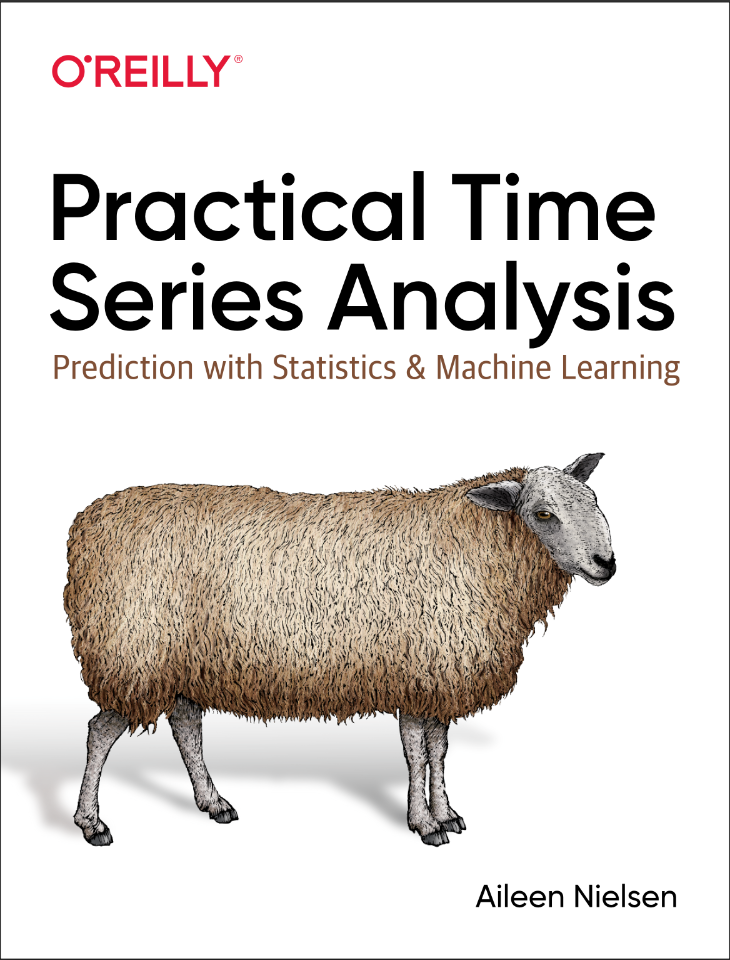
\includegraphics[width=0.9\linewidth]{Images/PTSA}
			\end{column}
			\begin{column}{0.60\textwidth}
				\textcite{nielsen2020practical} dedica um sub-capítulo em seu livro onde expõe que profissionais da indústria fazem conscientemente essa aplicação de modelos misspecificados por pragmatismo em troca de um resultado rápido.
				
				\vspace{0.2cm}
				\begin{quote}
					\small
					\textit{"Real-world analysts take liberties with model assumptions from time to time. This can be productive so long as the potential downsides of doing so are understood."}
				\end{quote}
			\end{column}
		\end{columns}
		
		\vspace{0.2cm}
		
		\footnotesize
		Portanto, a simplicidade só tem valor epistêmico quando acompanhada \\
		da \textbf{transparência} sobre o que ela sacrifica.

	\end{frame}
	

	\begin{frame}[allowframebreaks]{Referências}                                                                                                     
		\printbibliography[heading=none]                                                                                                                
	\end{frame}
      
\end{document}